\chapter{Observer}
\section{Intento}

Definisce un'interfaccia per la creazione di un oggetto, ma lasciare che le sottoclassi decidano quale classe istanziare.

(come l'Abstract Factory ma con un solo Product)


%---
\section{Struttura}

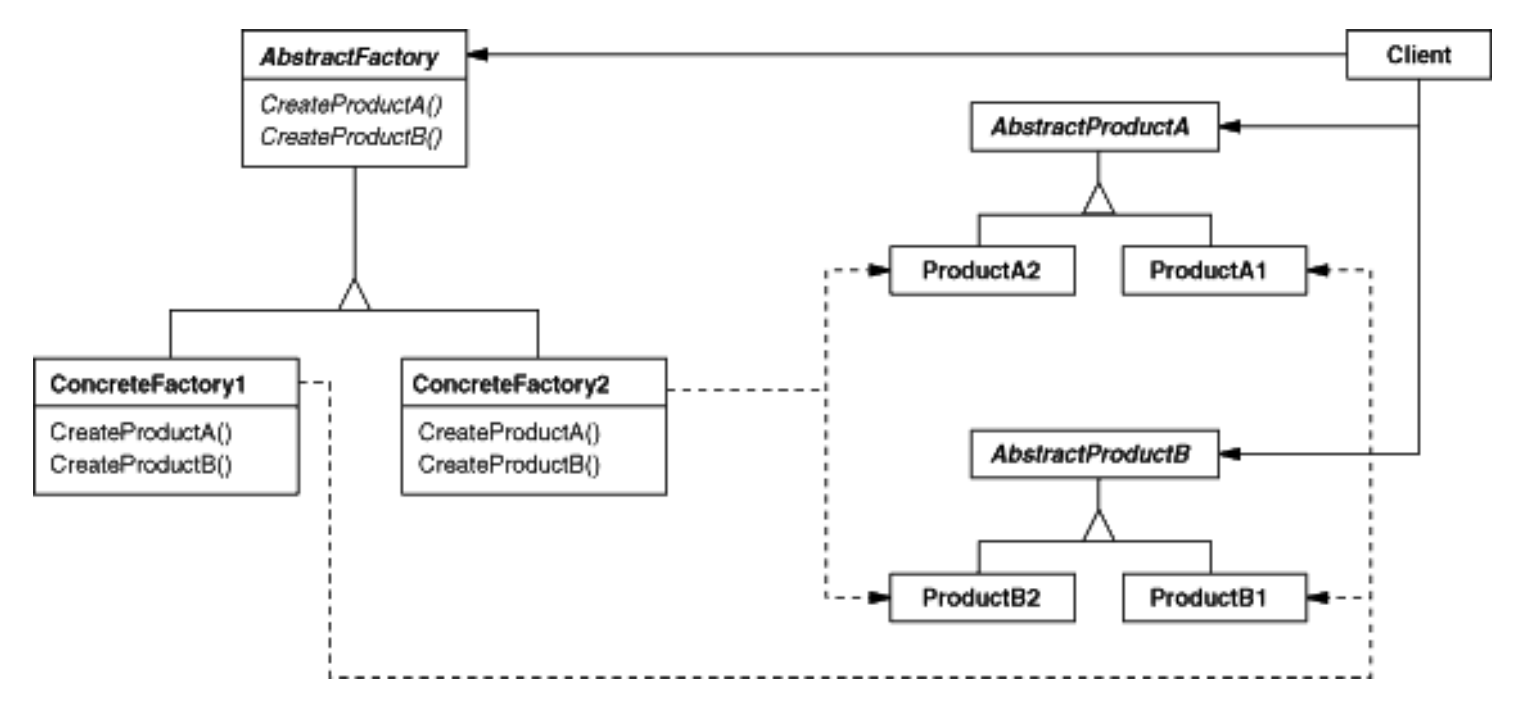
\includegraphics[width=\textwidth]{/Users/matt/Documents/LaTex/Design Pattern LaTex/Observer/Structure1}


%---
\section{Timeline}

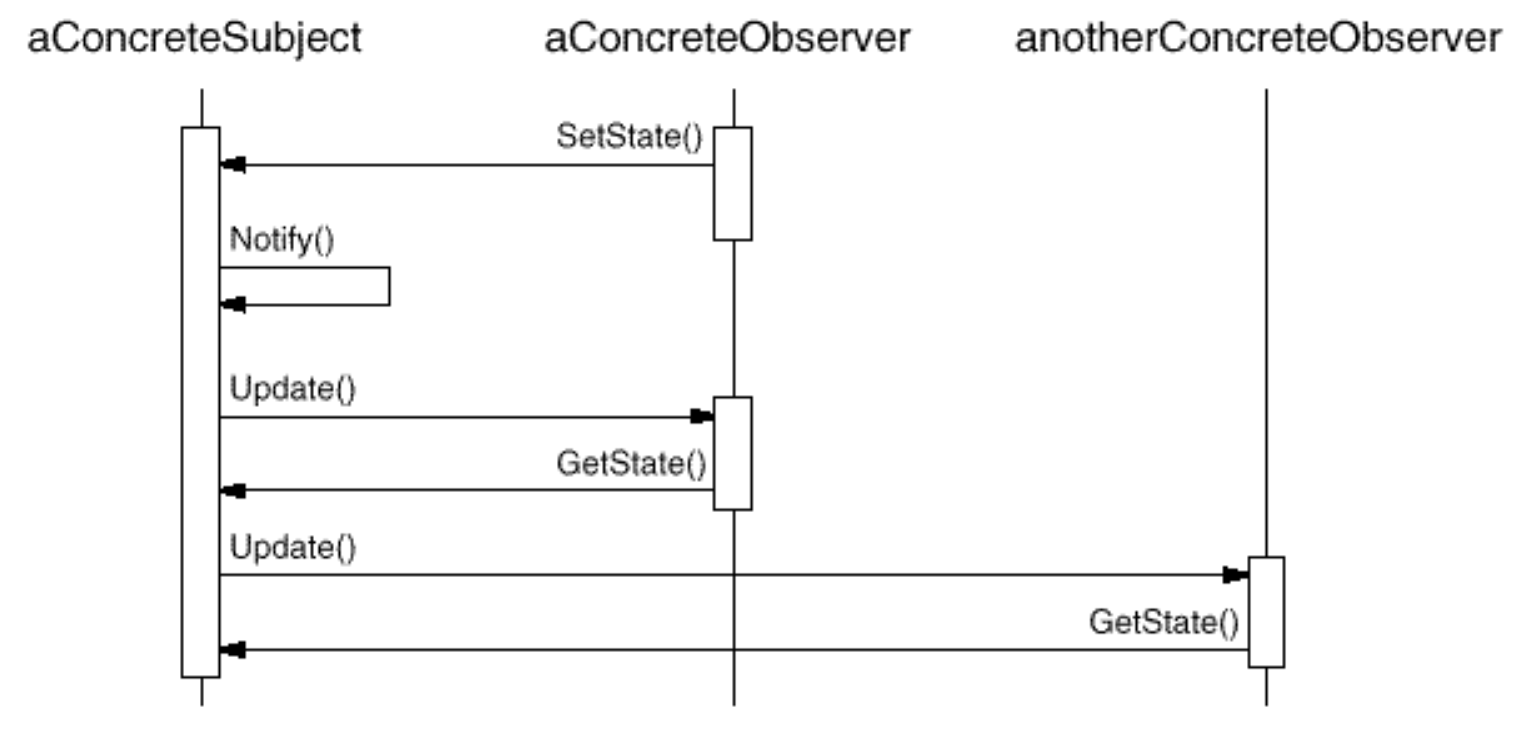
\includegraphics[width=\textwidth]{/Users/matt/Documents/LaTex/Design Pattern LaTex/Observer/Timeline1}


%---
\section{Implementazione}

\subsection{Mappare i soggetti ai loro osservatori.}
Tale archiviazione può essere troppo costosa quando ci sono molti soggetti e pochi osservatori.

Si può quindi utilizzare una ricerca associativa (ad esempio una tabella hash) per mantenere la mappatura soggetto-osservatore. Quindi un soggetto senza osservatori non incorre in spese di archiviazione.

\subsection{Osservare più di un soggetto.}
Potrebbe avere senso in alcune situazioni che un osservatore dipenda da più di un soggetto. 

In questi casi è necessario estendere l'interfaccia di aggiornamento per far sapere all'osservatore quale soggetto sta inviando la notifica (passando se stesso come parametro nell'operazione di aggiornamento, facendo sapere all'osservatore quale soggetto esaminare)

\subsection{Chi chiama Notify e attiva l'aggiornamento?}

\begin{itemize}
    \item Avere operazioni di impostazione dello stato sulla chiamata del soggetto Notifica dopo aver modificato lo stato del soggetto. 
        
    \begin{itemize}
        \item \textbf{Vantaggio}: i clienti non devono ricordarsi di chiamare Notify sull'argomento.

        \item \textbf{Svantaggio}: operazioni consecutive causano diversi aggiornamenti consecutivi. Potrebbe essere inefficiente.
    \end{itemize}

    \item Rendi i clienti responsabili di chiamare Notify al momento giusto.

    \begin{itemize}
        \item \textbf{Vantaggio}: il cliente ha la gestione degli aggiornamenti, evitando così inutili aggiornamenti. 

        \item \textbf{Svantaggio}: il cliente ha la responsabilità aggiuntiva di attivare l'aggiornamento, rendendo più probabili gli errori.
    \end{itemize}
\end{itemize}


\subsection{Riferimenti penzolanti a soggetti cancellati.}
Un modo per evitare riferimenti penzolanti è fare in modo che il soggetto informi i suoi osservatori quando viene cancellato in modo che possano reimpostare il loro riferimento ad esso.

La semplice eliminazione degli osservatori non è un'opzione, perché altri oggetti potrebbero fare riferimento a loro o potrebbero osservare anche altri soggetti.

\subsection{Assicurarsi che lo stato del soggetto sia coerente prima della notifica.}
È importante perché il soggetto è interrogato per il suo stato attuale nel corso dell'aggiornamento del proprio stato.
È facile da violare quando le operazioni della sottoclasse Oggetto chiamano operazioni ereditate.

È possibile evitarlo inviando notifiche dai Model in classi di soggetti astratte, facendo in modo che Notifica sia l'ultima operazione nel Model, che assicurerà che l'oggetto sia autoconsistente quando le sottoclassi sovrascrivono le operazioni del soggetto.

\subsection{Evitare protocolli di aggiornamento specifici dell'osservatore: i modelli push e pull.}
Le implementazioni del modello Observer spesso fanno trasmettere al soggetto informazioni aggiuntive sul cambiamento. Il soggetto passa queste informazioni come argomento ad Aggiorna. La quantità di informazioni può variare notevolmente.

\begin{itemize}
    \item \textbf{Modello PUSH}: presuppone che i soggetti sappiano qualcosa sui bisogni dei loro osservatori.

    I soggetti forniscono agli osservatori informazioni dettagliate sul cambiamento. (osservatori meno riutilizzabili)

    \item \textbf{Modello PULL}: enfatizza l'ignoranza del soggetto.
    
    Il soggetto invia la minima notifica e gli osservatori chiedono esplicitamente i dettagli in seguito. (può essere inefficiente)
\end{itemize}

\subsection{Specificazione esplicita delle modifiche di interesse.}
È possibile migliorare l'efficienza degli aggiornamenti consentendo la registrazione degli osservatori solo per eventi di interesse specifici. Per fare ciò sono attaccati ai loro soggetti usando

\begin{lstlisting}[language=java]
   void Attach(Osservatore, interesse);
\end{lstlisting}

Al momento della notifica, il soggetto fornisce l'aspetto modificato ai suoi osservatori. Per esempio:

\begin{lstlisting}[language=java]
   void Update(Subject, interesse);
\end{lstlisting}

\subsection{Incapsulamento di semantiche di aggiornamento complesse.}

\begin{itemize}
    \item \textbf{ChangeManager}: il suo scopo è ridurre al minimo il lavoro necessario per far riflettere gli osservatori su un cambiamento nel loro soggetto.
\end{itemize}

Ad esempio, se un'operazione comporta modifiche a più soggetti, potresti dover assicurarti che i loro osservatori vengano avvisati dopo che tutti i soggetti sono stati modificati per evitare di avvisare gli osservatori più di una volta.

ChangeManager ha tre responsabilità:

    \begin{enumerate}
        \item Mappa un soggetto ai suoi osservatori e fornisce un'interfaccia per mantenere questa mappatura. Ciò elimina la necessità per i soggetti di mantenere riferimenti ai propri osservatori e viceversa.

        \item Definisce una particolare strategia di aggiornamento.

        \item Aggiorna tutti gli osservatori dipendenti su richiesta di un soggetto.
    \end{enumerate}

Il DAGChangeManager assicura che l'osservatore riceva un solo aggiornamento. SimpleChangeManager va bene quando più aggiornamenti non sono un problema (il modello Singleton sarebbe utile qui).

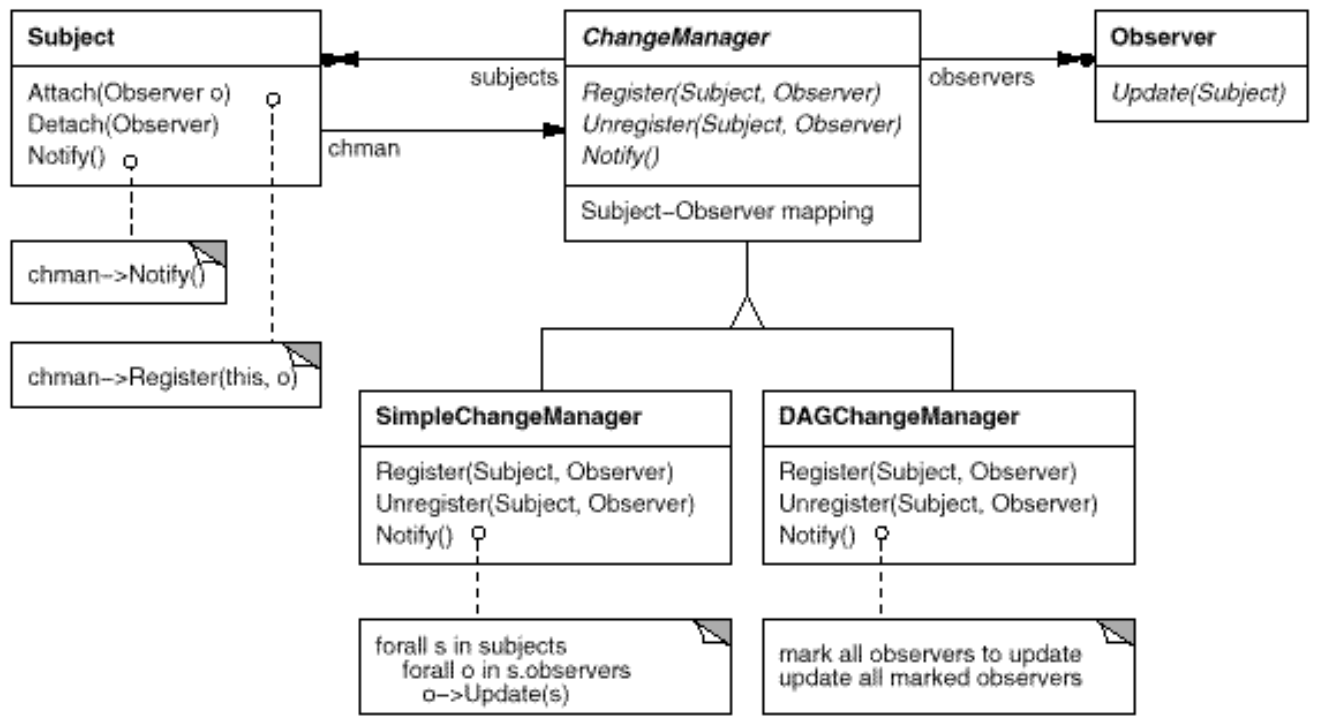
\includegraphics[width=\textwidth]{/Users/matt/Documents/LaTex/Design Pattern LaTex/Observer/ChangeManager}


%---
\section{Esempio Java}
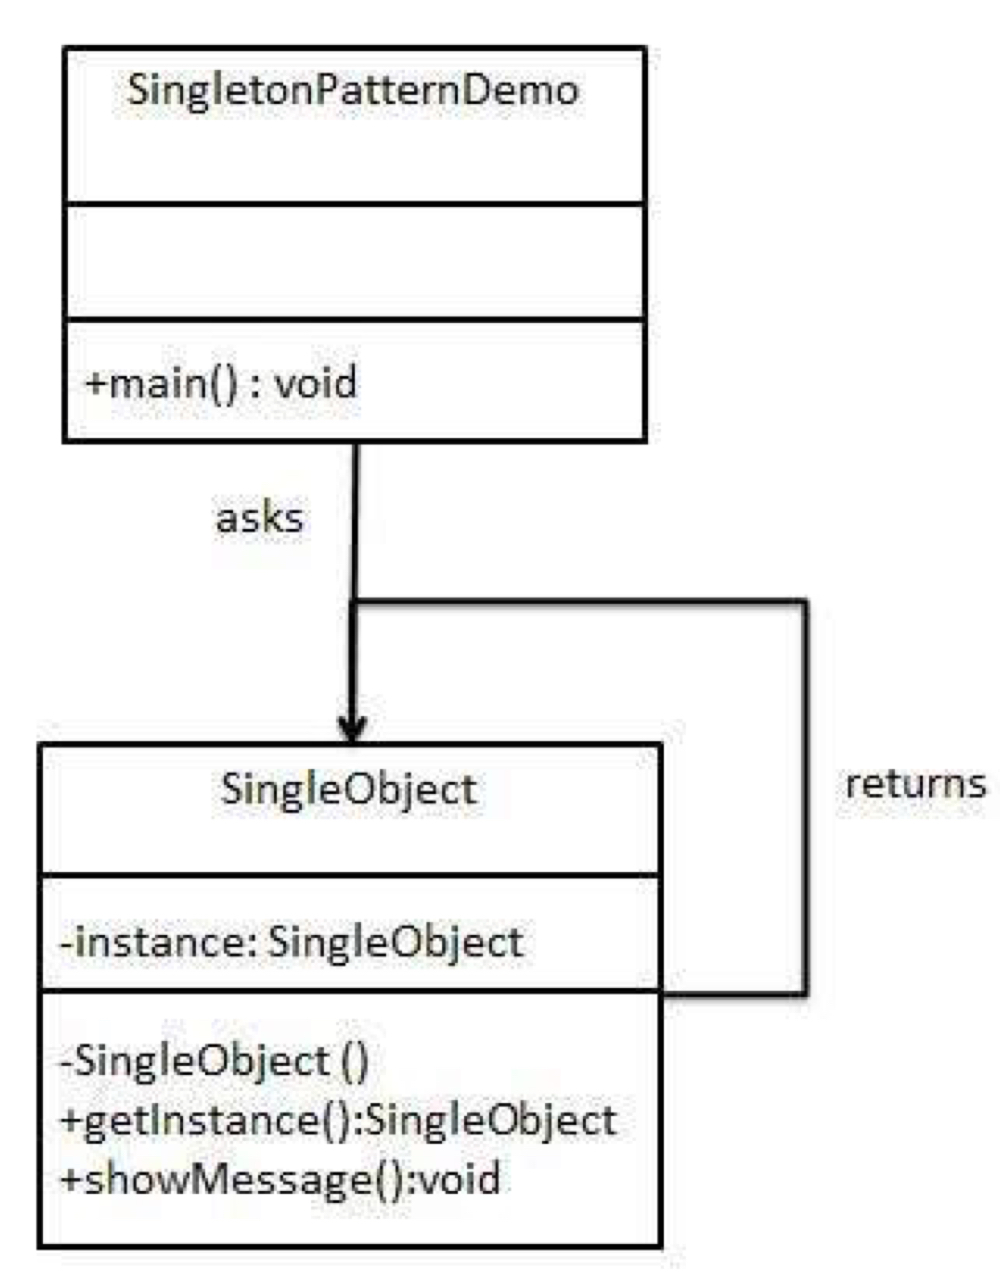
\includegraphics[width=\textwidth]{/Users/matt/Documents/LaTex/Design Pattern LaTex/Observer/Example1}

\subsection{ClickListener.java}
\begin{lstlisting}[language=java]
    public class ClickListener implements ActionListener {

        @Override
        public void actionPerformed(ActionEvent e) {
            JButton bc = (JButton) e.getSource();
            if (bc.getText().equals("Cliccato")) {
                bc.setText("Decliccato");
            } else {
                bc.setText("Cliccato");
            }
        }
    }
\end{lstlisting}

\subsection{main}
\begin{lstlisting}[language=java]
    public static void main(String[] args) {
        /** 
         * Creazione del frame e del pulsante
         */  
        JFrame f = new JFrame();
        JButton b = new JButton("Decliccato");

        /** 
         * Si aggiunge al frame il pulsante
         */ 
        f.add(b);

        /** 
         * Creazione di un Ascoltatore di Azioni
         *  per andare a notificare i cambiamenti alla view
         */
        ActionListener al = new ClickListener();

        /**    !!! PARTE IMPORTANTE PER L'OBSERVER !!!
         * Si aggiunge al pulsante l'ActionListener
         *  in modo che i due siano collegati
         */
        b.addActionListener(al);

        /**
         * Setting del frame
         */
        f.setSize(300, 200);
        f.setDefaultCloseOperation(JFrame.EXIT_ON_CLOSE);
        f.setVisible(true);
    }
\end{lstlisting}